% !TeX program = xelatex
% 2025 年普通高等学校招生全国统一考试（新课标 I 卷）数学 —— 解析版
% 编译方式：XeLaTeX，需要 exam-zh 宏包（TeX Live 2020+）
\documentclass{exam-zh}
\usepackage{tikz}
\usepackage{diagbox}
\examsetup{
  question/show-answer = true,
  solution/show-solution = show-stay,
}

\begin{document}

\begin{center}
  {\zihao{3}\bfseries 2025 年普通高等学校招生全国统一考试（新课标 \uppercase\expandafter{\romannumeral1} 卷）}\\[4pt]
  {\zihao{4}\bfseries 数\quad 学（解析版）}
\end{center}

\section{选择题：本题共 8 小题，每小题 5 分，共 40 分。在每小题给出的四个选项中，只有一项是符合题目要求的。}

\begin{question}
$(1+5\iu)\iu$ 的虚部为 \paren[C]
\begin{choices}
  \item $-1$
  \item $0$
  \item $1$
  \item $6$
\end{choices}
\begin{solution}
因为 $(1+5\iu)\iu=\iu+5\iu^{2}=-5+\iu$，所以其虚部为 $1$。故选 C。
\end{solution}
\end{question}

\begin{question}
设全集 $U=\{x\mid x\text{ 是小于 }9\text{ 的正整数}\}$，集合 $A=\{1,3,5\}$，则 $\complement_{U}A$ 中元素个数为 \paren[C]
\begin{choices}
  \item $0$
  \item $3$
  \item $5$
  \item $8$
\end{choices}
\begin{solution}
$U=\{1,2,3,4,5,6,7,8\}$，故 $\complement_{U}A=\{2,4,6,7,8\}$，共 $5$ 个元素。故选 C。
\end{solution}
\end{question}

\begin{question}
若双曲线 $C$ 的虚轴长为实轴长的 $\sqrt{7}$ 倍，则 $C$ 的离心率为 \paren[D]
\begin{choices}
  \item $\sqrt{2}$
  \item $2$
  \item $\sqrt{7}$
  \item $2\sqrt{2}$
\end{choices}
\begin{solution}
设实轴长、虚轴长分别为 $2a$、$2b$，由题知 $b=\sqrt{7}a$。于是 $c^{2}=a^{2}+b^{2}=a^{2}+7a^{2}=8a^{2}$，则 $c=2\sqrt{2}a$，即 $e=\dfrac{c}{a}=2\sqrt{2}$。故选 D。
\end{solution}
\end{question}

\begin{question}
若点 $(a,0)\,(a>0)$ 是函数 $y=2\tan\left(x-\dfrac{\uppi}{3}\right)$ 的图象的一个对称中心，则 $a$ 的最小值为 \paren[C]
\begin{choices}
  \item $\dfrac{\uppi}{4}$
  \item $\dfrac{\uppi}{2}$
  \item $\dfrac{\uppi}{3}$
  \item $\dfrac{4\uppi}{3}$
\end{choices}
\begin{solution}
正切函数 $y=2\tan\left(x-\dfrac{\uppi}{3}\right)$ 的对称中心横坐标满足 $x-\dfrac{\uppi}{3}=\dfrac{k\uppi}{2}\,(k\in\mathbb{Z})$，即对称中心为 $\left(\dfrac{\uppi}{3}+\dfrac{k\uppi}{2},0\right)$，故 $a=\dfrac{\uppi}{3}+\dfrac{k\uppi}{2}\,(k\in\mathbb{Z})$。又 $a>0$，当 $k=0$ 时 $a$ 最小，最小值为 $\dfrac{\uppi}{3}$。故选 C。
\end{solution}
\end{question}

\begin{question}
设 $f(x)$ 是定义在 $\mathbb{R}$ 上且周期为 $2$ 的偶函数，当 $2\le x\le 3$ 时，$f(x)=5-2x$，则 $f\left(-\dfrac{3}{4}\right)=$ \paren[A]
\begin{choices}
  \item $-\dfrac{1}{2}$
  \item $-\dfrac{1}{4}$
  \item $\dfrac{1}{4}$
  \item $\dfrac{1}{2}$
\end{choices}
\begin{solution}
由偶函数与周期性，$f\left(-\dfrac{3}{4}\right)=f\left(\dfrac{3}{4}\right)=f\left(\dfrac{3}{4}+2\right)=f\left(\dfrac{11}{4}\right)=5-2\times\dfrac{11}{4}=-\dfrac{1}{2}$。故选 A。
\end{solution}
\end{question}

\begin{question}
帆船比赛中，运动员可借助风力计测定风速的大小和方向，测出的结果在航海学中称为视风速。视风速对应的向量，是真风速对应的向量与船行风速对应的向量之和，其中船行风速对应的向量与船速对应的向量大小相同，方向相反。图 1 给出了部分风力等级、名称与风速大小的对应关系。已知某帆船运动员在某时刻测得的视风风速对应的向量与船速对应的向量如图 2（风速的大小和向量的大小相同），单位（m/s），则真风为 \paren[A]

\begin{center}
\begin{tabular}{|c|c|c|}
\hline
等级 & 风速大小 m/s & 名称 \\
\hline
2 & $1.1\sim 3.3$ & 轻风 \\
\hline
3 & $3.4\sim 5.4$ & 微风 \\
\hline
4 & $5.5\sim 7.9$ & 和风 \\
\hline
5 & $8.0\sim 10.1$ & 劲风 \\
\hline
\end{tabular}

\vspace{4pt}{\footnotesize 图 1}
\end{center}

\begin{center}
\begin{tikzpicture}[scale=0.85,>=stealth]
  \draw[->](0,0)--(4,0)node[right]{$x$};
  \draw[->](0,0)--(0,4)node[above]{$y$};
  \foreach \i in {1,2,3}{
    \draw(\i,0.08)--(\i,-0.08)node[below]{\scriptsize$\i$};
    \draw(0.08,\i)--(-0.08,\i)node[left]{\scriptsize$\i$};}
  \draw[->,very thick](0,0)--(3,3);
  \node at (1.1,2.2){\footnotesize 视风风速};
  \draw[->,very thick](2,1)--(3,3);
  \node at (2.8,1.5){\footnotesize 船速};
  \draw[dashed](2,0)--(2,1)--(0,1);
  \node[below left] at (0,0){\scriptsize $O$};
  \node at (1.7,-0.6){\footnotesize 图 2};
\end{tikzpicture}
\end{center}

\begin{choices}
  \item 轻风
  \item 微风
  \item 和风
  \item 劲风
\end{choices}
\begin{solution}
设真风速对应的向量为 $\vec{n_{1}}$，船行风速对应的向量为 $\vec{n_{2}}$，则视风速向量 $\vec{n}=\vec{n_{1}}+\vec{n_{2}}$。由图及题意求出真风速对应的向量 $\vec{n_{1}}=(-2,2)$，则真风速的大小 $|\vec{n_{1}}|=\sqrt{(-2)^{2}+2^{2}}=2\sqrt{2}\approx 2.828\ \text{m/s}$。对照图 1 可知真风速为轻风。故选 A。
\end{solution}
\end{question}

\begin{question}
若圆 $x^{2}+(y+2)^{2}=r^{2}\,(r>0)$ 上到直线 $y=\sqrt{3}x+2$ 的距离为 $1$ 的点有且仅有 $2$ 个，则 $r$ 的取值范围是 \paren[B]
\begin{choices}
  \item $(0,1)$
  \item $(1,3)$
  \item $(3,+\infty)$
  \item $(0,+\infty)$
\end{choices}
\begin{solution}
圆心 $E(0,-2)$，半径 $r$。圆心到直线 $\sqrt{3}x-y+2=0$ 的距离
\[d=\frac{|0\times\sqrt{3}-(-2)+2|}{\sqrt{(\sqrt{3})^{2}+(-1)^{2}}}=\frac{4}{2}=2.\]
结合图象：当 $r=1$ 时，圆上到该直线距离为 $1$ 的点有且仅有 $1$ 个；当 $r=3$ 时有且仅有 $3$ 个；当 $r\in(1,3)$ 时有且仅有 $2$ 个。故选 B。
\end{solution}
\end{question}

\begin{question}
若实数 $x,y,z$ 满足 $2+\log_{2}x=3+\log_{3}y=5+\log_{5}z$，则 $x,y,z$ 的大小关系不可能是 \paren[B]
\begin{choices}
  \item $x>y>z$
  \item $x>z>y$
  \item $y>x>z$
  \item $y>z>x$
\end{choices}
\begin{solution}
令 $2+\log_{2}x=3+\log_{3}y=5+\log_{5}z=m$，则 $x=2^{m-2}$，$y=3^{m-3}$，$z=5^{m-5}$。

取 $m=2$：$x=1$，$y=\dfrac13$，$z=\dfrac1{125}$，此时 $x>y>z$，A 可能；取 $m=5$：$x=8$，$y=9$，$z=1$，此时 $y>x>z$，C 可能；取 $m=8$：$x=64$，$y=243$，$z=125$，此时 $y>z>x$，D 可能。由指数函数的单调性作图可知，随着 $m$ 的变化可能出现 $x>y>z$，$y>x>z$，$y>z>x$，$z>y>x$，唯独 $x>z>y$ 不可能。故选 B。
\end{solution}
\end{question}

\section{选择题：本题共 3 小题，每小题 6 分，共 18 分。在每小题给出的选项中，有多项符合题目要求。全部选对的得 6 分，部分选对的得部分分，有选错的得 0 分。}

\begin{question}
在正三棱柱 $ABC\text{-}A_{1}B_{1}C_{1}$ 中，$D$ 为 $BC$ 中点，则 \paren[BC]
\begin{choices}
  \item $AD\perp A_{1}C$
  \item $BC\perp$ 平面 $AA_{1}D$
  \item $CC_{1}\parallel$ 平面 $AA_{1}D$
  \item $AD\parallel A_{1}B_{1}$
\end{choices}
\begin{solution}
$AA_{1}\perp$ 平面 $ABC$，$D$ 为 $BC$ 中点，则 $AD\perp BC$。

对于 A：$\overrightarrow{A_{1}C}=\overrightarrow{A_{1}A}+\overrightarrow{AD}+\overrightarrow{DC}$，则 $\overrightarrow{A_{1}C}\cdot\overrightarrow{AD}=\overrightarrow{AD}^{2}\ne 0$，故 $AD\perp A_{1}C$ 不成立，A 错误；

对于 B：$AA_{1}\perp BC$，$AD\perp BC$，$AA_{1}\cap AD=A$，故 $BC\perp$ 平面 $AA_{1}D$，B 正确；

对于 C：$CC_{1}\parallel AA_{1}$，$AA_{1}\subset$ 平面 $AA_{1}D$，$CC_{1}\not\subset$ 平面 $AA_{1}D$，故 $CC_{1}\parallel$ 平面 $AA_{1}D$，C 正确；

对于 D：若 $AD\parallel A_{1}B_{1}$，则 $AD\parallel AB$，与 $AD\cap AB=A$ 矛盾，D 错误。故选 BC。
\end{solution}
\end{question}

\begin{question}
设抛物线 $C\colon y^{2}=6x$ 的焦点为 $F$，过 $F$ 的直线交 $C$ 于 $A$、$B$，过 $F$ 且垂直于 $AB$ 的直线交 $l\colon x=-\dfrac{3}{2}$ 于 $E$，过点 $A$ 作准线 $l$ 的垂线，垂足为 $D$，则 \paren[ACD]
\begin{choices}
  \item $|AD|=|AF|$
  \item $|AE|=|AB|$
  \item $|AB|\ge 6$
  \item $|AE|\cdot|BE|\ge 18$
\end{choices}
\begin{solution}
抛物线 $y^{2}=6x$ 中 $p=3$，准线 $x=-\dfrac32$，焦点 $F\left(\dfrac32,0\right)$。

A：$|AD|$ 为 $A$ 到准线的距离，由抛物线定义 $|AD|=|AF|$，正确；

B：可证 $\angle AEB\ne 0$，$AE$ 不等于斜边 $AB$，故 $|AE|=|AB|$ 不成立，错误；

C：设 $AB\colon x=my+\dfrac32$，与 $y^{2}=6x$ 联立得 $y^{2}-6my-9=0$，$y_{1}+y_{2}=6m$，$y_{1}y_{2}=-9$，则 $|AB|=x_{1}+x_{2}+p=m(y_{1}+y_{2})+3+3=6m^{2}+6\ge 6$（$m=0$ 时取等号），正确；

D：由 $\mathrm{Rt}\triangle ABE\sim\mathrm{Rt}\triangle AEF$ 得 $|AE|^{2}=|AF|\cdot|AB|$，同理 $|BE|^{2}=|BF|\cdot|AB|$，于是 $|AE|\cdot|BE|=|AB|\sqrt{|AF|\cdot|BF|}$。经计算 $|AE|\cdot|BE|=18\left(1+\dfrac1{k^{2}}\right)^{\frac32}\ge 18$（或斜率不存在时 $=18$），正确。故选 ACD。
\end{solution}
\end{question}

\begin{question}
已知 $\triangle ABC$ 的面积为 $\dfrac{1}{4}$，若 $\cos 2A+\cos 2B+2\sin C=2$，$\cos A\cos B\sin C=\dfrac{1}{4}$，则 \paren[ABC]
\begin{choices}
  \item $\sin C=\sin^{2}A+\sin^{2}B$
  \item $AB=\sqrt{2}$
  \item $\sin A+\sin B=\dfrac{\sqrt{6}}{2}$
  \item $AC^{2}+BC^{2}=3$
\end{choices}
\begin{solution}
由二倍角公式，$\cos 2A+\cos 2B+2\sin C=1-2\sin^{2}A+1-2\sin^{2}B+2\sin C=2$，整理得 $\sin C=\sin^{2}A+\sin^{2}B$，A 正确。

由 $\sin C=\sin^{2}A+\sin^{2}B$ 及 $\sin C=\sin(A+B)$ 可推出 $A+B=\dfrac{\uppi}{2}$，即 $C=\dfrac{\uppi}{2}$。于是 $\sin C=1$，$\cos A\cos B=\dfrac14$。又 $A+B=\dfrac{\uppi}{2}$，$\cos B=\sin A$，则 $\cos A\sin A=\dfrac12\sin 2A=\dfrac14$，$\sin 2A=\dfrac12$。不妨设 $A<B$，则 $2A=\dfrac{\uppi}{6}$，$2B=\dfrac{5\uppi}{6}$，即 $A=\dfrac{\uppi}{12}$，$B=\dfrac{5\uppi}{12}$。

由两角差、两角和的正弦公式，$\sin A+\sin B=\sin\dfrac{\uppi}{12}+\sin\dfrac{5\uppi}{12}=\dfrac{\sqrt6-\sqrt2}{4}+\dfrac{\sqrt6+\sqrt2}{4}=\dfrac{\sqrt6}{2}$，C 正确。

设 $BC=a$，$AC=b$，则 $ab\cdot\dfrac12\sin C=\dfrac14$，$ab=\dfrac12$；结合 $\tan\dfrac{5\uppi}{12}=2+\sqrt3$ 求得 $AB=c=\sqrt2$，B 正确。由勾股定理 $AC^{2}+BC^{2}=c^{2}=2\ne 3$，D 错误。故选 ABC。
\end{solution}
\end{question}

\section{填空题：本题共 3 小题，每小题 5 分，共 15 分。}

\begin{question}
若直线 $y=2x+5$ 是曲线 $y=\eu^{x}+x+a$ 的切线，则 $a=$ \fillin[4] 。
\begin{solution}
对 $y=\eu^{x}+x+a$ 求导得 $y'=\eu^{x}+1$。由切线斜率为 $2$，令 $\eu^{x}+1=2$，解得 $x=0$。将 $x=0$ 代入切线 $y=2x+5$ 得切点 $(0,5)$。因为切点在曲线上，所以 $5=\eu^{0}+0+a=1+a$，解得 $a=4$。
\end{solution}
\end{question}

\begin{question}
若一个等比数列的前 $4$ 项和为 $4$，前 $8$ 项和为 $68$，则该等比数列的公比为 \fillin[{$\pm 2$}] 。
\begin{solution}
设公比为 $q$。若 $q=1$，则 $S_{8}=2S_{4}$，与 $S_{8}=68\ne 8$ 矛盾，舍去。当 $q\ne 1$ 时，$\dfrac{S_{8}}{S_{4}}=\dfrac{1-q^{8}}{1-q^{4}}=1+q^{4}=\dfrac{68}{4}=17$，解得 $q^{4}=16$，即 $q=\pm 2$。故公比为 $\pm 2$。
\end{solution}
\end{question}

\begin{question}
一个箱子里有 $5$ 个相同的球，分别以 $1\sim 5$ 标号，若有放回地取三次，记至少取出一次的球的个数 $X$，则数学期望 $E(X)=$ \fillin[{$\dfrac{61}{25}$}] 。
\begin{solution}
对每个球，其在三次抽取中未被取出的概率为 $\left(\dfrac45\right)^{3}=\dfrac{64}{125}$，故至少被取出一次的概率为 $1-\dfrac{64}{125}=\dfrac{61}{125}$。记第 $i$ 个球被取出记为 $X_{i}=1$，否则 $X_{i}=0$，则 $X=\sum_{i=1}^{5}X_{i}$，由期望的线性性得
\[E(X)=\sum_{i=1}^{5}E(X_{i})=5\times\dfrac{61}{125}=\dfrac{61}{25}.\]
\end{solution}
\end{question}

\section{解答题：本题共 5 小题，共 77 分。解答应写出文字说明、证明过程或演算步骤。}

\begin{problem}[points = 13]
为研究某疾病与超声波检查结果的关系，从做过超声波检查的人群中随机调查了 $1000$ 人，得到如下列联表：

\begin{center}
\begin{tabular}{|c|c|c|c|}
\hline
\diagbox{组别}{超声波检查结果} & 正常 & 不正常 & 合计 \\
\hline
患该疾病 & $20$ & $180$ & $200$ \\
\hline
未患该疾病 & $780$ & $20$ & $800$ \\
\hline
合计 & $800$ & $200$ & $1000$ \\
\hline
\end{tabular}
\end{center}

（1）记超声波检查结果不正常者患该疾病的概率为 $P$，求 $P$ 的估计值；

（2）根据小概率值 $\alpha=0.001$ 的独立性检验，分析超声波检查结果是否与患该疾病有关。

附 $\chi^{2}=\dfrac{n(ad-bc)^{2}}{(a+b)(c+d)(a+c)(b+d)}$，

\begin{center}
\begin{tabular}{|c|c|c|c|}
\hline
$P(\chi^{2}\ge k)$ & $0.050$ & $0.010$ & $0.001$ \\
\hline
$k$ & $3.841$ & $6.635$ & $10.828$ \\
\hline
\end{tabular}
\end{center}

\begin{solution}
（1）检查结果不正常的 $200$ 人中有 $180$ 人患病，故 $P$ 的估计值为 $\dfrac{180}{200}=\dfrac{9}{10}$。

（2）零假设 $H_{0}$：超声波检查结果与患该疾病无关。根据表中数据，
\[\chi^{2}=\frac{1000\times(20\times 20-780\times 180)^{2}}{200\times 800\times 800\times 200}=765.625>10.828=x_{0.001}.\]
依据小概率值 $\alpha=0.001$ 的独立性检验，推断 $H_{0}$ 不成立，即认为超声波检查结果与患该疾病有关，该推断犯错误的概率不超过 $0.001$。
\end{solution}
\end{problem}

\begin{problem}[points = 15]
设数列 $\{a_{n}\}$ 满足 $a_{1}=3$，$\dfrac{a_{n+1}}{n}=\dfrac{a_{n}}{n+1}+\dfrac{1}{n(n+1)}$。

（1）证明：$\{na_{n}\}$ 为等差数列；

（2）设 $f(x)=a_{1}x+a_{2}x^{2}+\cdots+a_{m}x^{m}$，求 $f'(-2)$。

\begin{solution}
（1）在 $\dfrac{a_{n+1}}{n}=\dfrac{a_{n}}{n+1}+\dfrac{1}{n(n+1)}$ 两边同乘 $n(n+1)$，得 $(n+1)a_{n+1}=na_{n}+1$，即 $(n+1)a_{n+1}-na_{n}=1$。故 $\{na_{n}\}$ 是以 $a_{1}=3$ 为首项、$1$ 为公差的等差数列。

（2）由（1），$na_{n}=3+1\times(n-1)=n+2$，即 $a_{n}=1+\dfrac{2}{n}$。于是
\[f(x)=3x+2x^{2}+\cdots+\left(1+\dfrac{2}{m}\right)x^{m},\quad f'(x)=3+4x+5x^{2}+\cdots+(m+2)x^{m-1}.\]
两式作差（错位相减）：$xf'(x)=3x+4x^{2}+\cdots+(m+2)x^{m}$，故当 $x\ne 1$ 时
\[(1-x)f'(x)=3+x+x^{2}+\cdots+x^{m-1}-(m+2)x^{m}=3+\frac{x(1-x^{m-1})}{1-x}-(m+2)x^{m},\]
\[f'(x)=\frac{3}{1-x}+\frac{x\left(1-x^{m-1}\right)}{(1-x)^{2}}-\frac{(m+2)x^{m}}{1-x}.\]
代入 $x=-2$：
\[f'(-2)=1+\frac{-2\left[1-(-2)^{m-1}\right]}{9}-\frac{(m+2)(-2)^{m}}{3}=\frac{7}{9}-\frac{(3m+7)(-2)^{m}}{9}.\]
\end{solution}
\end{problem}

\begin{problem}[points = 15]
如图所示的四棱锥 $P\text{-}ABCD$ 中，$PA\perp$ 平面 $ABCD$，$BC\parallel AD$，$AB\perp AD$。

\begin{center}
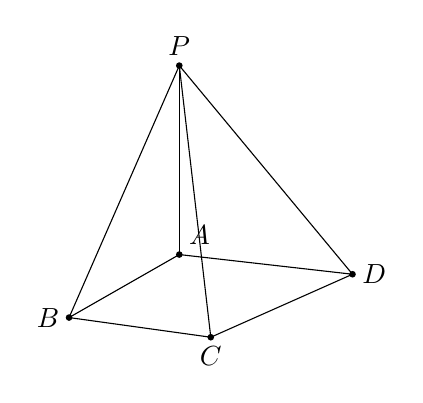
\begin{tikzpicture}[scale=1.0,>=stealth]
  \coordinate (A) at (0,0);
  \coordinate (B) at (-1.4,-0.8);
  \coordinate (C) at (0.4,-1.05);
  \coordinate (D) at (2.2,-0.25);
  \coordinate (P) at (0,2.4);
  \draw (A)--(B)--(C)--(D)--(A);
  \draw (P)--(A); \draw (P)--(B); \draw (P)--(C); \draw (P)--(D);
  \foreach \pt/\pos in {A/{above right},B/{left},C/{below},D/{right},P/{above}}
    \fill (\pt) circle (1.2pt) node[\pos]{$\pt$};
\end{tikzpicture}
\end{center}

（1）证明：平面 $PAB\perp$ 平面 $PAD$；

（2）$PA=AB=\sqrt{2}$，$AD=1+\sqrt{3}$，$BC=2$，$P$、$B$、$C$、$D$ 在同一个球面上，设该球面的球心为 $O$。

\qquad（i）证明：$O$ 在平面 $ABCD$ 上；

\qquad（ii）求直线 $AC$ 与直线 $PO$ 所成角的余弦值。

\begin{solution}
（1）因为 $PA\perp$ 平面 $ABCD$，$AB$、$AD\subset$ 平面 $ABCD$，所以 $PA\perp AB$，$PA\perp AD$。又 $AB\perp AD$，$PA\cap AD=A$，故 $AB\perp$ 平面 $PAD$。而 $AB\subset$ 平面 $PAB$，所以平面 $PAB\perp$ 平面 $PAD$。

（2）（i）以 $A$ 为原点，$AB$、$AD$、$AP$ 方向为 $x$、$y$、$z$ 轴建立空间直角坐标系，则
\[A(0,0,0),\ B(\sqrt{2},0,0),\ C(\sqrt{2},2,0),\ D(0,1+\sqrt{3},0),\ P(0,0,\sqrt{2}).\]
设球心 $O(x_{0},y_{0},0)$，由 $|OP|=|OB|=|OC|=|OD|$ 解得 $O(0,1,0)$，且 $|OP|=|OB|=|OC|=|OD|=\sqrt{3}$。故点 $O$ 在线段 $AD$ 上，即 $O$ 在平面 $ABCD$ 上。

（ii）$\overrightarrow{AC}=(\sqrt{2},2,0)$，$\overrightarrow{PO}=(0,1,-\sqrt{2})$。设直线 $AC$ 与 $PO$ 所成角为 $\theta$，则
\[\cos\theta=\frac{\left|\overrightarrow{AC}\cdot\overrightarrow{PO}\right|}{\left|\overrightarrow{AC}\right|\left|\overrightarrow{PO}\right|}=\frac{|0+2+0|}{\sqrt{(\sqrt{2})^{2}+2^{2}}\times\sqrt{0+1^{2}+(-\sqrt{2})^{2}}}=\frac{2}{\sqrt{6}\times\sqrt{3}}=\frac{\sqrt{2}}{3}.\]
\end{solution}
\end{problem}

\begin{problem}[points = 17]
设椭圆 $C\colon \dfrac{x^{2}}{a^{2}}+\dfrac{y^{2}}{b^{2}}=1\,(a>b>0)$ 的离心率为 $\dfrac{2\sqrt{2}}{3}$，下顶点为 $A$，右顶点为 $B$，$|AB|=\sqrt{10}$。

（1）求椭圆的标准方程；

（2）已知点 $P$ 不在 $y$ 轴上，点 $R$ 在射线 $AP$ 上，且满足 $|AR|\cdot|AP|=3$。

\qquad（i）设 $P(m,n)$，求点 $R$ 的坐标（用 $m$、$n$ 表示）；

\qquad（ii）设 $O$ 为坐标原点，$M$ 是椭圆上的动点，直线 $OR$ 的斜率是直线 $OP$ 的斜率的 $3$ 倍，求 $|PM|$ 的最大值。

\begin{solution}
（1）$A(0,-b)$，$B(a,0)$，由 $|AB|=\sqrt{a^{2}+b^{2}}=\sqrt{10}$，$e=\dfrac{c}{a}=\dfrac{2\sqrt{2}}{3}$ 及 $c^{2}=a^{2}-b^{2}$，解得 $a^{2}=9$，$b^{2}=1$，$c^{2}=8$。故椭圆的标准方程为 $\dfrac{x^{2}}{9}+y^{2}=1$。

（2）（i）$A(0,-1)$，设 $R(x_{0},y_{0})$，$m\ne 0$。$R$ 在射线 $AP$ 上，$\dfrac{y_{0}+1}{x_{0}}=\dfrac{n+1}{m}$ 且 $mx_{0}>0$。由 $|AR|\cdot|AP|=3$，即 $\sqrt{x_{0}^{2}+(y_{0}+1)^{2}}\cdot\sqrt{m^{2}+(n+1)^{2}}=3$，联立解得 $x_{0}=\dfrac{3m}{m^{2}+(n+1)^{2}}$，$y_{0}=\dfrac{n+2-m^{2}-n^{2}}{m^{2}+(n+1)^{2}}$。故
\[R\left(\frac{3m}{m^{2}+(n+1)^{2}},\ \frac{n+2-m^{2}-n^{2}}{m^{2}+(n+1)^{2}}\right).\]

（ii）$k_{OR}=\dfrac{y_{0}}{x_{0}}=\dfrac{n+2-m^{2}-n^{2}}{3m}$，$k_{OP}=\dfrac{n}{m}$。由 $k_{OR}=3k_{OP}$ 得 $\dfrac{n+2-m^{2}-n^{2}}{3m}=\dfrac{3n}{m}$，化简得 $m^{2}+n^{2}+8n-2=0$，即 $m^{2}+(n+4)^{2}=18$（$m\ne 0$）。所以点 $P$ 在以 $N(0,-4)$ 为圆心、$3\sqrt{2}$ 为半径的圆上（除去两点）。

$|PM|$ 的最大值为 $M$ 到圆心 $N$ 的距离加上半径。设 $M(3\cos\theta,\sin\theta)$，则
\[|MN|^{2}=(3\cos\theta)^{2}+(\sin\theta+4)^{2}=-8\sin^{2}\theta+8\sin\theta+25=-8\left(\sin\theta-\dfrac12\right)^{2}+27\le 27,\]
当 $\sin\theta=\dfrac12$ 时取等号，故 $|MN|_{\max}=\sqrt{27}=3\sqrt{3}$。所以 $|PM|_{\max}=3\sqrt{3}+3\sqrt{2}=3(\sqrt{3}+\sqrt{2})$。
\end{solution}
\end{problem}

\begin{problem}[points = 17]
设函数 $f(x)=5\cos x-\cos 5x$。

（1）求 $f(x)$ 在 $\left[0,\dfrac{\uppi}{4}\right]$ 的最大值；

（2）给定 $\theta\in(0,\uppi)$，设 $a$ 为实数，证明：存在 $y\in[a-\theta,a+\theta]$，使得 $\cos y\le\cos\theta$；

（3）若存在 $\varphi$ 使得对任意 $x$，都有 $5\cos x-\cos(5x+\varphi)\le b$，求 $b$ 的最小值。

\begin{solution}
（1）$f'(x)=-5\sin x+5\sin 5x=10\cos 3x\sin 2x$。当 $x\in\left(0,\dfrac{\uppi}{4}\right)$ 时 $\sin 2x>0$；当 $0<x<\dfrac{\uppi}{6}$ 时 $\cos 3x>0$，$f'(x)>0$，当 $\dfrac{\uppi}{6}<x<\dfrac{\uppi}{4}$ 时 $\cos 3x<0$，$f'(x)<0$。故 $f(x)$ 在 $\left(0,\dfrac{\uppi}{6}\right)$ 上递增，在 $\left(\dfrac{\uppi}{6},\dfrac{\uppi}{4}\right)$ 上递减，最大值为
\[f\left(\dfrac{\uppi}{6}\right)=5\cos\dfrac{\uppi}{6}-\cos\dfrac{5\uppi}{6}=\dfrac{5\sqrt{3}}{2}+\dfrac{\sqrt{3}}{2}=3\sqrt{3}.\]

（2）由余弦函数的性质，不等式 $\cos y\le\cos\theta$ 的解集为 $\bigcup_{k\in\mathbb{Z}}[2k\uppi+\theta,\,2k\uppi+2\uppi-\theta]$。假设对任意 $k\in\mathbb{Z}$，区间 $[2k\uppi+\theta,\,2k\uppi+2\uppi-\theta]$ 与 $[a-\theta,a+\theta]$ 的交集均为空，则需 $a-\theta>2k\uppi+2\uppi-\theta$ 且 $a+\theta<2(k+1)\uppi+\theta$ 对每个 $k$ 之一成立，这要求长度为 $1$ 的相关区间上不含满足条件的整数 $k$，与整数的存在性矛盾。故存在 $k$ 使两区间相交，即存在 $y\in[a-\theta,a+\theta]$ 使得 $\cos y\le\cos\theta$。

（3）$b$ 的最小值为 $3\sqrt{3}$。

记 $h(x)=5\cos x-\cos(5x+t)$，它是周期为 $2\uppi$ 的函数。一方面，若存在 $t$ 使 $g_{t}(x)=5\cos x-\cos(5x+t)\le b$ 对任意 $x$ 恒成立，由 $g_{t}(x+\uppi)=-g_{t}(x)$ 可得 $|g_{t}(x)|\le b$ 恒成立，从而 $b\ge 0$；进一步结合 $\cos 2x=2\cos^{2}x-1$ 的取值分析（三个角 $2m,\,2m+\dfrac{2\uppi}{3},\,2m-\dfrac{2\uppi}{3}$ 对应单位圆上三等分点，不可能都在 $x=\dfrac12$ 左侧）可证 $b\ge 3\sqrt{3}$。

另一方面，取 $\varphi=0$，由（1）已证 $5\cos x-\cos 5x=f(x)\le 3\sqrt{3}$，故 $b=3\sqrt{3}$ 满足题目要求。综上，$b_{\min}=3\sqrt{3}$。
\end{solution}
\end{problem}

\end{document}
